\documentclass[11pt, oneside]{article}   	% use "amsart" instead of "article" for AMSLaTeX format
\usepackage{geometry}                		% See geometry.pdf to learn the layout options. There are lots.
\geometry{letterpaper}                   		% ... or a4paper or a5paper or ... 
%\geometry{landscape}                		% Activate for rotated page geometry
%\usepackage[parfill]{parskip}    		% Activate to begin paragraphs with an empty line rather than an indent
\usepackage{graphicx}				% Use pdf, png, jpg, or eps§ with pdflatex; use eps in DVI mode
								% TeX will automatically convert eps --> pdf in pdflatex		
\usepackage{amssymb}
\usepackage{amsmath}
\usepackage{dcolumn}
\usepackage[table, svgnames, x11names]{xcolor}

\addtolength{\oddsidemargin}{-.875in}
	\addtolength{\evensidemargin}{-.875in}
	\addtolength{\textwidth}{1.75in}

	\addtolength{\topmargin}{-.875in}
	\addtolength{\textheight}{1.75in}



\newcolumntype{d}[1]{D{.}{.}{#1}}

%SetFonts

%SetFonts


\title{Computational modeling}
\author{Nicolas P. Cottaris}
\date{}							% Activate to display a given date or no date

\begin{document}
\maketitle
\section{ISETBio computational model}
\subsection{Overview}
To connect the measured RGC spatial transfer functions (STF) to the underlying retinal anatomy, a computational model is employed which simulates optical, spectral, spatial, and temporal components of the AO stimulation apparatus, as well as the monkey's optics and cone mosaic structure. The model computes an STF, assuming that cone signals are pooled by the center and surround mechanisms of an RGC according to a difference of Gaussians (DoG) spatial profile model. The parameters of the DoG model and therefore, the actual cone pooling weights, are estimating by minimizing the error between the predicted and measured STFs. A schematic overview of this model is depicted in Figure \ref{fig:ModelOverview}. Various model parameters used to simulate various aspects of the experimental conditions are listed in Table \ref{table:ModelParameters}.

\subsection{AO-delivered stimulus modeling}
The AO-delivered drifting monochromatic sinusoidal gratings used to measured RGC STFs during the experiment, are modeled as temporal sequences of ISETBio spatial spectral radiance scenes, where each scene models a different frame of the drifting stimulus. The spectral profile of the monochromatic beam, the spatial extent and resolution, and the temporal characteristic of the AO display subsystem as are all taken into account in generating these scenes. 

\subsection{Retinal stimulus modeling}
The generated scenes are subsequently passed via a diffraction-limited optical system model which accounts for blur in optical in a perfect AO system and which can also account for additional residual amount blur that may occur in a slightly imperfect AO system, for example due to a slight defocus of the stimulus with respect to the plane of cone inner segments. (Say something more here??). The amount of residual blur in not known a-priori, and it is estimated from the model as described below. 

\subsection{Cone excitation response modeling}
In the next stage, an ISETBio model of the monkey's cone mosaic is generated using an iterative approach [Cottaris et al] from cone density maps measured during AO imaging. The temporal photon absorption excitation response, $E^j(\omega,t)$, of each cone-$j$ of the mosaic, to a drifting grating of spatial frequency $\omega$, is computed from the corresponding temporal sequence of retinal spatial spectral irradiance images, after weighing retinal irradiance by each cone's spectral quantal efficiency and spatially integrating the result within each cone's inner segment aperture. 

\subsection{Converting cone excitation responses to cone contrast responses}
Assuming that cones are adapted to the mean background irradiance, the excitation response of a cone-$j$ to a stimulus with spatial frequency $\omega$, $E^j(\omega,t)$, is converted to contrast response, $R^j(\omega, t)$, by first subtracting the excitation to the background stimulus, $E^j_o$, and then dividing by it, separately for each cone-$j$, i.e.:
\begin{equation}
R^j(\omega, t) = \frac{E^j(\omega,t) - E^j_o}{E^j_o}
\end{equation}
\noindent where
$E^j_o$ is the excitation of cone-$j$, to the zero contrast (background) stimulus. This operation mimics the photocurrent generation process which converts cone absorption events in the inner segment into ionic currents flowing through the cone outer segment, and which in effect normalizes stimulus-induced cone excitations responses with respect to the background cone excitation responses.
Eye movements are assumed to be zero, since the AO apparatus effectively stabilizes stimuli on the retina.


\subsection{Computing model ganglion cells responses}
Model ganglion cells responses, $\mbox{RGC}(\omega,t)$, are computed from the cone contrast responses assuming linear spatial pooling of cone contrast signals by the antagonistic center and the surround mechanisms, as follows:
\begin{eqnarray}
\mbox{RGC}(\omega,t) & = & \mbox{RGC}_c(\omega,t) - \mbox{RGC}_s(\omega,t) \\
& = & \sum_{j} W_{c}^j  \times R^j(\omega, t) -  \sum_{j} W_{s}^j  \times R^j(\omega, t)
\end{eqnarray}
%
\noindent where, $W_{c}^j, W_{s}^j$, are the spatial pooling weights with which the center and surround, respectively, mechanisms are summing the $R^j(\omega, t)$ responses. There is no temporal filtering, and no delay is introduced in the computation of center, $\mbox{RGC}_c(\omega,t)$, and surround $\mbox{RGC}_s(\omega,t)$ responses. 

\subsection{Computing model RGC spatial transfer functions}
The STF of a model RGC, $\mbox{STF}^{m}(\omega)$, is computed as: 
\begin{equation}
\mbox{STF}^{m}(\omega) = \mbox{STF}_{c}^{m}(\omega) - \mbox{STF}_{s}^{m}(\omega)
\end{equation}
%
\noindent with
%
\begin{eqnarray}
\mbox{STF}_{c}^{m}(\omega) & = &\max_{t} \left \{ \mbox{RGC}_c(\omega,t)  \right \} \\ 
\mbox{STF}_{s}^{m}(\omega) & = &\max_{t} \left \{ \mbox{RGC}_s(\omega,t)  \right \}
\end{eqnarray}


\subsection{Estimating cone pooling weights from the fluorescence-based STF measurements}

The weights with which the center and surround mechanisms of a model RGC, are pooling signals from a cone-$j$ are computed as follows:
\begin{eqnarray}
W_c^j  & = & \begin{cases}
   k_c \times \exp \left [ -\left( d_{j}/r_c \right) ^2 \right ], & \text{for the multi-cone RF center model}.\\
   k_c, & \text{for the single-cone RF center model}.
   \end{cases} \\
W_s^j &= &k_s \times \exp \left [ -\left( d_{j}/r_s \right) ^2 \right ]
\end{eqnarray}

\noindent where $d_j$ is the distance between cone-$j$ and the spatial position of the center mechanism of the model RGC. The parameters $k_c$, $k_s$, $r_c$ and $r_s$ are determined by minimizing the weighted error between the model STF, $\mbox{STF}^{m}(\omega)$, and the measured STF, $\mbox{STF}^{\Delta F / F}(\omega)$, over all spatial frequencies, $\omega$:

\begin{equation}
\mbox{RMSE} = \displaystyle \sum_{\omega} \frac{1}{\epsilon({\omega})} {\left [  \mbox{STF}^{m}(\omega)  - \mbox{STF}^{\Delta F / F}(\omega) \right ] }^2
\end{equation}
where $\epsilon({\omega})$ is the standard error of the mean of the $\mbox{STF}^{\Delta F / F}(\omega)$ measurement. To minimize the chance of getting stuck to local minima of the error function, we employ a multi-start minimizer which is ran 1024 times, keeping the results from the run which results in the minimum rms error.

Since the receptive field location of the recorded RGCs is only known approximately to lie within the central 40 $\mu m$, we repeat the above analysis a number of times, each time assuming that the model RGC receives its center-driving signal from cones in different parts of the central 40 $\mu m$ of the model cone mosaic. 


\subsection{Model validation}
To validate the extracted RF model parameters ($k_c$, $k_s$, $r_c$ and $r_s$), we employ a cross-validation approach, in which we train the model by minimizing the error with respect to the $\mbox{STF}^{\Delta F / F}$ measured in one recording session (in-sample error), and assess model performance by quantifying the error with respect to the $\mbox{STF}^{\Delta F / F}$ measured at the remaining recording sessions (out-of-sample error). Therefore, we run as many cross-validation assessments as there are recording sessions, each time training the model on a different session, $s_i$, and computing the average cross-validated error across the remaining sessions, $s_j \ne s_i$, $\mbox{RMSE}_{train = s_1\dots s_n}^{s_j \ne s_i}$. The selected model is the one with the minimal  cross-validated error. This analysis is repeated for each of the assumed receptive field center positions, and the final $k_c$, $k_s$, $r_c$ and $r_s$ values are chosen to be those which minimize the cross-validated error across all examined RF center positions.

This cross-validation approach allows us to determine $k_c$, $k_s$, $r_c$ and $r_s$ model parameters with the maximal generalization potential, which are less likely to be prone to overfitting the training data set. This approach is also used to compare performance across models with different number of parameters, for example the single-cone RF center model, where the $r_c$ parameter is absent (in effect fixed to the underlying cone characteristic radius), vs. the multi-cone RF center model, where the $r_c$ parameter is allowed to vary.

\newpage


\begin{table}% put at top of page if possible 
\centering
\begin{tabular}{|r d{3.3}|}
%\begin{tabular}{|r l|}
\hline
\rowcolor{LightSlateGray!35!Lavender} \multicolumn{2}{|l|}{\textbf{retinal modeling (optics)}} \\
\hline
\mbox{pupil diameter} ($mm$) : & 6.7  \\
\mbox{retinal magnification factor} ($\mu m \times deg^{-1}$) : & 199.26 \\
\hline
\hline
\rowcolor{LightSlateGray!35!Lavender} \multicolumn{2}{|l|}{\textbf{retinal modeling (cone mosaic)}} \\
\hline
\mbox{size} (degs) : & \multicolumn{1}{c|}{1.3 $\times$ 1.3}\\
\mbox{max. density} ($10^3 \mbox{cones} \times mm^{-2}$) : & 270.20\\  
\mbox{cone aperture profile} : & \multicolumn{1}{c|}{\mbox{Gaussian}}\\
\mbox{cone aperture characteristic radius} : & \multicolumn{1}{c|}{0.204 $\times \sqrt{2} \times$
\mbox{i.s. diam.}}\\
\mbox{foveal cone characteristic radius (arc.min.)} : & \multicolumn{1}{c|}{0.17}\\
\mbox{L-cone ratio} : & \multicolumn{1}{c|}{0.48}\\
\mbox{M-cone ratio} : & \multicolumn{1}{c|}{0.48}\\
\mbox{S-cone ratio} : & \multicolumn{1}{c|}{0.04}\\
\hline
\hline
\rowcolor{LightSlateGray!35!Lavender}  \multicolumn{2}{|l|}{\textbf{visual stimulation modeling}} \\
\hline
\mbox{monochromatic stimulation (peak)} ($nm$) : & 561.0  \\
\mbox{monochromatic stimulation (FWHM)} ($nm$) : & 5.0  \\
\mbox{retinal pixel size} ($\mu m$) : & 1.03  \\
\mbox{drift rate} ($Hz$) : & 6.0  \\
\mbox{refresh rate} ($Hz$) : & 25.3  \\
\mbox{spatial extent} ($degs$) : & \multicolumn{1}{c|}{0.7 $\times$ 0.7}\\
\mbox{mean power} ($mW \times cm^2$) : & 1.29  \\
\mbox{contrast} : & 1.0 \\
\hline
\end{tabular}
\caption{Modeling parameters}\label{table:ModelParameters}
\end{table}


\begin{figure}[htbp] %  figure placement: here, top, bottom, or page
   \centering
   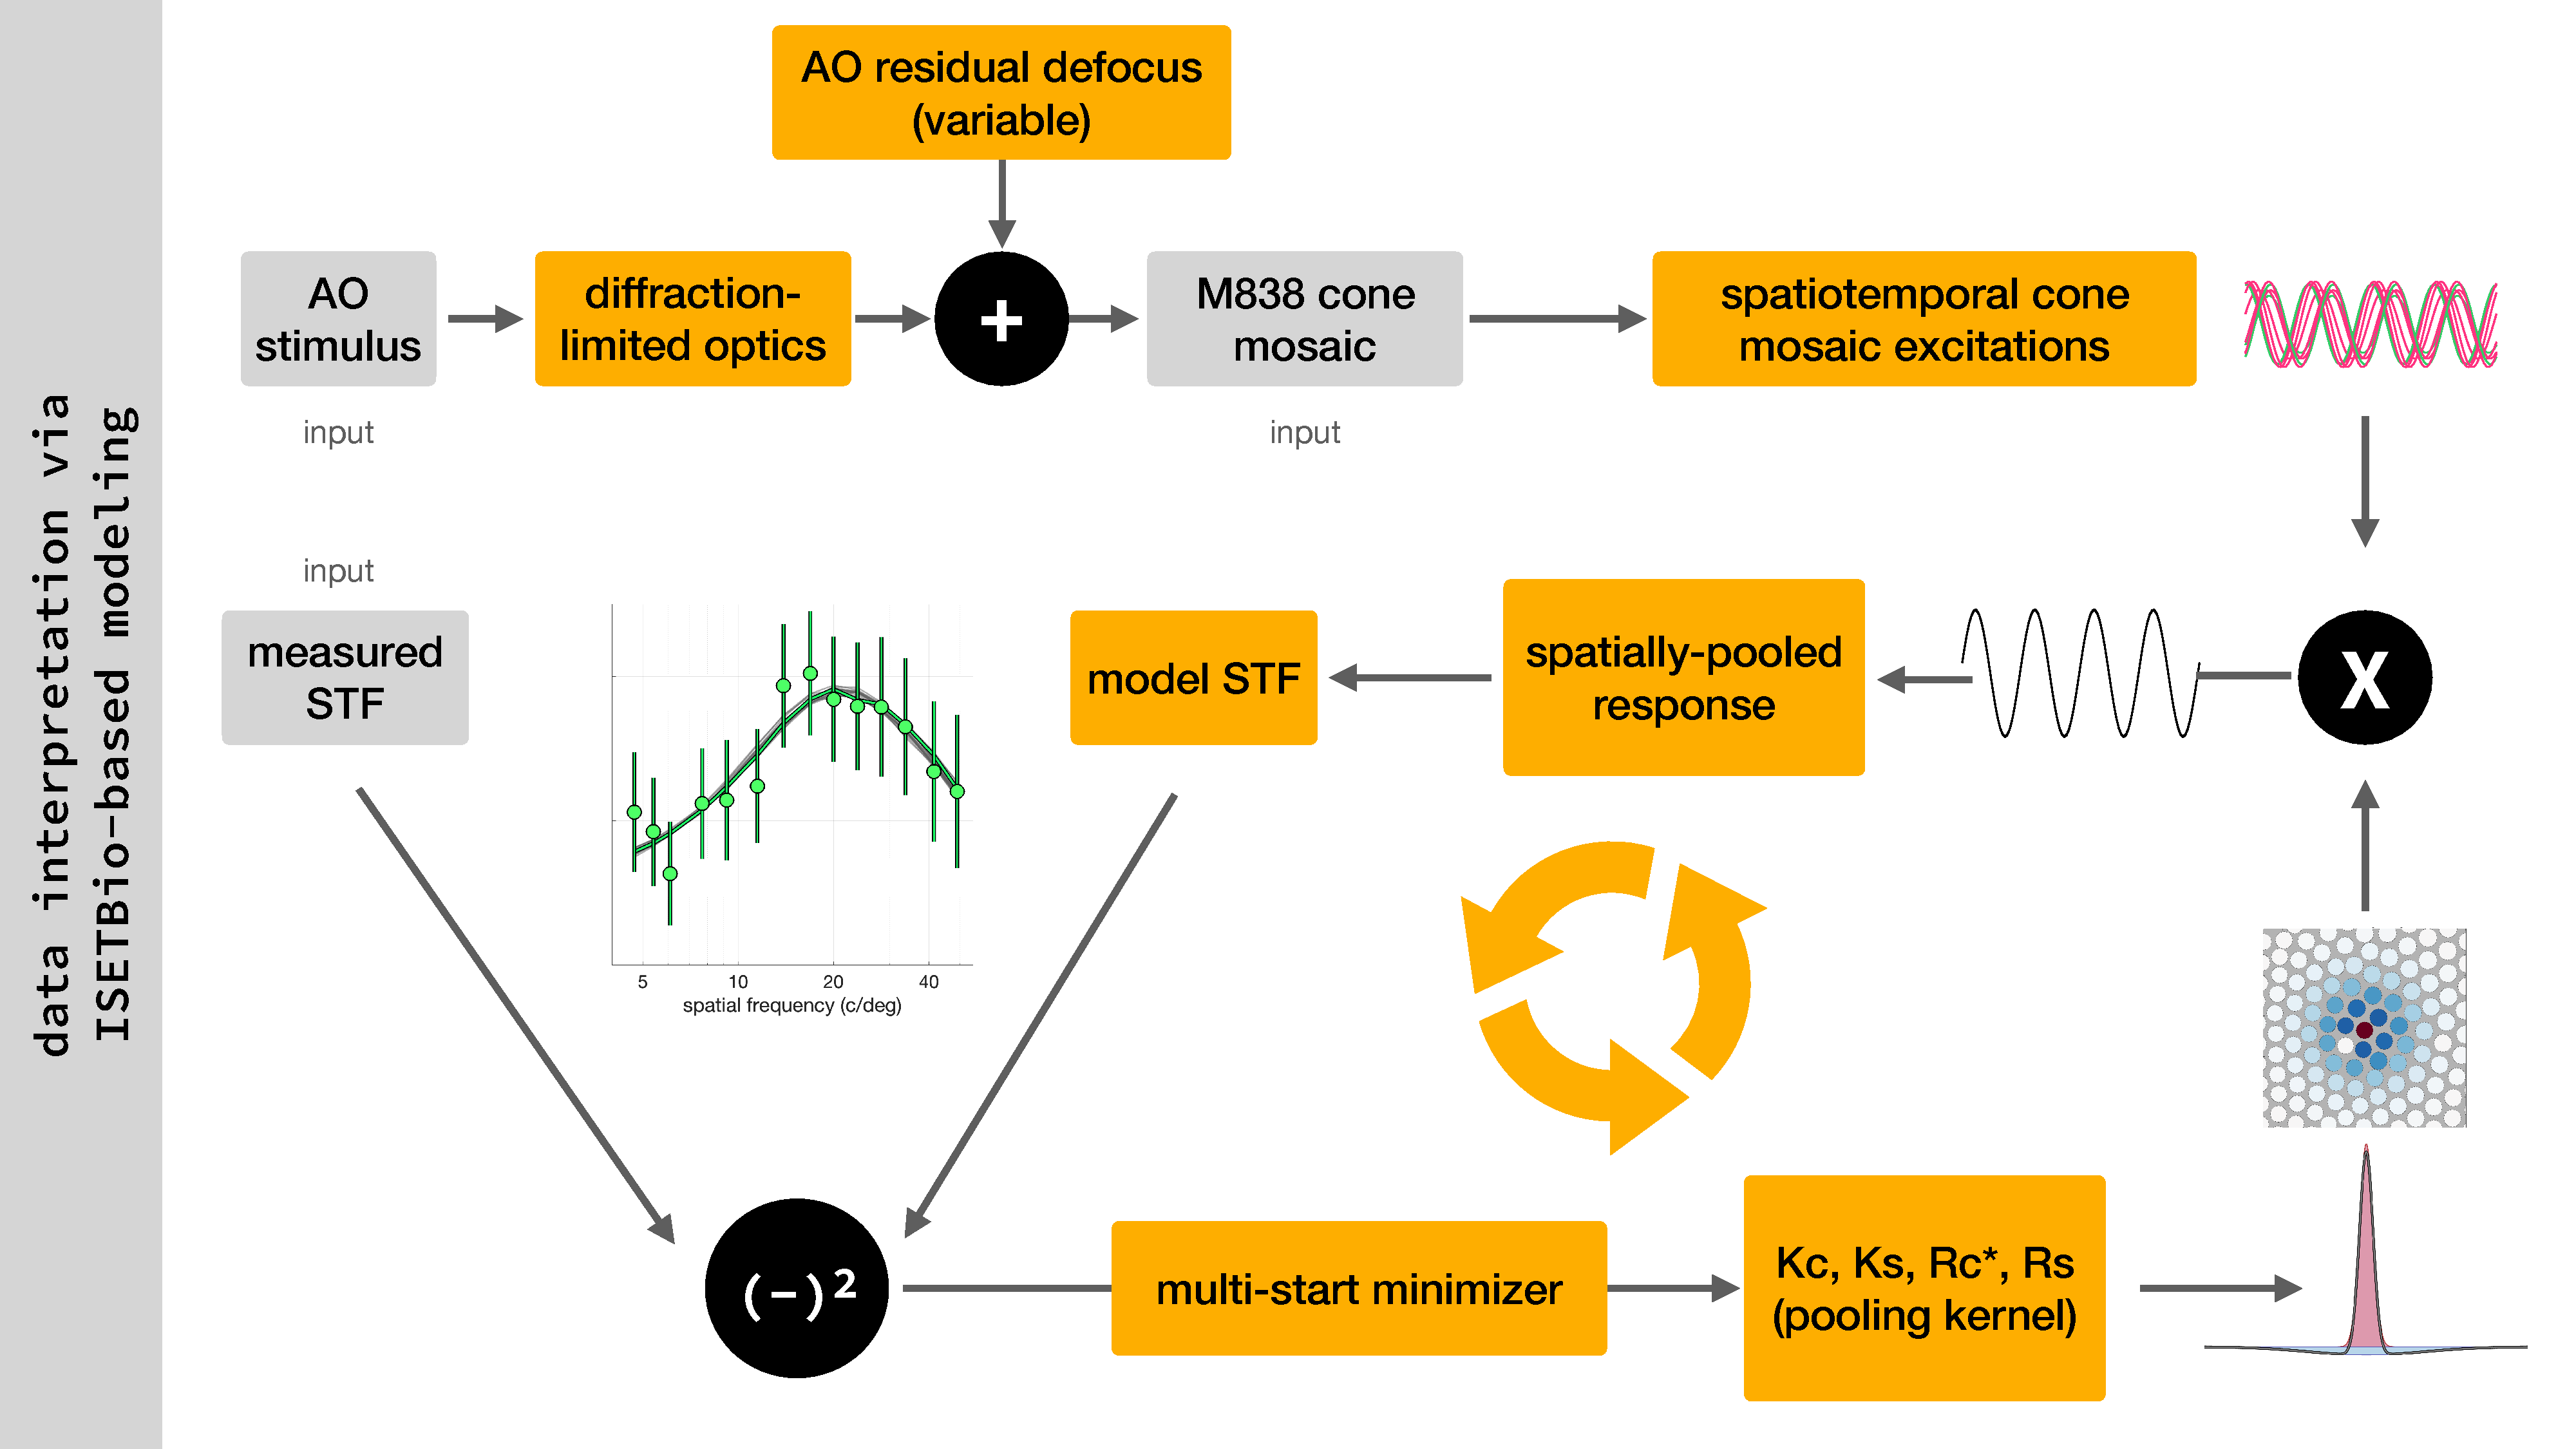
\includegraphics[width=7in]{Figures/ModelOverview.pdf} 
   \caption{Schematic overview of the ISETBio computational model.}
   \label{fig:ModelOverview}
\end{figure}



\end{document}  